%%「論文」,「レター」,「レター(C分冊)」,「技術研究報告」などのテンプレート
%% 1. 「論文」
%% v3.0 [2015/11/14]
\documentclass[paper]{ieicej}
%\documentclass[invited]{ieicej}% 招待論文
%\documentclass[survey]{ieicej}% サーベイ論文
%\documentclass[comment]{ieicej}% 解説論文
%\usepackage[dvips]{graphicx}
\usepackage[dvipdfmx]{graphicx,xcolor}
\usepackage[T1]{fontenc}
\usepackage{lmodern}
\usepackage{textcomp}
\usepackage{latexsym}
%\usepackage[fleqn]{amsmath}
%\usepackage{amssymb}
\usepackage{subfigure}

\setcounter{page}{1}

\field{}
\jtitle{PEGマシンのFPGA実装について}
\etitle{}
\authorlist{%
 \authorentry{マイ マイクオン}{Mai MaiCuong}{横浜国立大学}\MembershipNumber{}
 \authorentry{本多峻}{Honda Shun}{横浜国立大学}\MembershipNumber{}
 \authorentry{倉光君郎}{Kuramitsu Kimio}{横浜国立大学}\MembershipNumber{}
 %\authorentry[メールアドレス]{和文著者名}{英文著者名}{所属ラベル}\MembershipNumber{}
 %\authorentry{和文著者名}{英文著者名}{所属ラベル}[現在の所属ラベル]\MembershipNumber{}
}
\affiliate[]{}{}
%\affiliate[所属ラベル]{和文所属}{英文所属}
%\paffiliate[]{}
%\paffiliate[現在の所属ラベル]{和文所属}

\begin{document}
\begin{abstract}
解析表現文法(PEG)は、2004年にFordによって提案された形式文法であり、
正規表現や文脈自由文法の代替として人気が高まっている。
本稿では、より高い性能要求を目指すため、PEGのFPGA実装、
特にPEG演算子の仮想マシン化によるバーチャルマシン方式について報告し、
性能に関する初期レポートを行う予定である。
\end{abstract}
\begin{keyword}
%和文キーワード 4〜5語
\end{keyword}
\begin{eabstract}
%英文アブストラクト 100 words
\end{eabstract}
\begin{ekeyword}
%英文キーワード
\end{ekeyword}
\maketitle

\section{まえがき}

近年、クラウドなどのデータセンターで使うコンピューティングデバイスとして性能向上や電力削減の期待から、FPGAが注目されている。例えば、Microsoft社がWebエンジン「Bing]の処理を高速化するために、自社のデータセンターFPGAを導入すると発表した。また、中国のネット検索サービス大手のBaidu社も画像検索サービスの実装にFPGAの導入を検討している。Intel社でもサーバーCPU「Xeon]のパッケージにFPGAを収める製品を投入する予定である。\\
データセンターでは、ウイルス対策などのセキュリティ対策が不可欠である。その対策の一つとして、侵入検知システム(IDS:Instruction Detection System)がある。IDSでは、ネットワーク型とホスト型がある。ネットワーク型は、通常の振る舞いとの比較により、不正アクセスを検知するため、処理が重い。一方、ホスト型は既存の不正アクセスパターンを記憶し、パターンマッチングにより、不正アクセスを検知する。そのため、ホスト型の処理は比較的に軽く、現在侵入検知システムとして普及している。\\
現在ホスト型は、既存の不正アクセスパターンを正規表現で記述することが多い。しかし、パターンの複雑度に従い、パターンマッチング回路が大きくなることは問題である。\\
本研究では、パターンに依存せず、コンパクトなマッチングマシンを実現することを目的としている。そのため、解析表現文法(Parsing Expression Grammar)を用いる。PEGはFordによって提案され、正規表現や文脈自由文法の代替として人気が高まっている。


%構文解析とは、定義された文法に従ってテキストの構造を解析することである。この技術はプログラミング言語処理系のみならず、現在Web Page(HTMLやXML)の読み込みやTwitterつぶやきの解析、通信パケットの不正検出など、あらゆる場面で活用されている。現在構文解析を実現するために、正規表現や文脈自由文法という形式文法が広く用いられている。\\

%一方、2004年に解析表現文法(Parsing Expression Grammar)はFordによって提案され、正規表現や文脈自由文法の代替として人気が高まっている(PEG論文)。PEGはPackrat Parsing(PP論文)により線形時間に解析することができる。しかし、Packratは大きな入力に対して莫大なメモリ容量を使用するため、大きなデータの分析に向いていない。そこで、大きな入力を受理するため、MedeirosがPEGのためのVirtual Parsing Machineを提案した(VM論文)。PEGファイルを一つのプログラムに変換して、Virtual Machineで実行される。\\

%一方、近年、IoT(Intenet of things)の発展につれ、様々な機器への組み込みやすさやより高度なパケット処理が必要になった。また、ビックデータ時代になった今は、より高速な構文解析技法が求められている。そのため、組み込みやすさと高速な処理の面から、FPGAが注目されている。構文解析分野でも、FPGAを用いる研究がいくつかある。例えば、文脈自由文法を使ってFPGA上の構文解析\cite{CFG}やFPGA上で正規表現を用いたパターンマッチングマシン\cite{RE1}などの研究がある。\\

%正規表現論文()では、正規表現のマッチングマシンを作るには、3ステップが必要である。まず正規表現を木構造に変換し、次に非決定オートマトンに変換する。非決定オートマトンに変換する際、HDLに変換しやすいように、修正したMcNaughton構造を提案した。最後に非決定オートマトンからHDLに変換する。修正したMcNaughton構造を採用することより、コンパクトな構造が実現できた。一方、文脈自由文法論文()では、文脈自由文法を解析するために、Cocke-Younger-Kasamiアルゴリズムを用いた。\\

%本稿では、より高い性能要求を目指すため、PEGのFPGA実装、特にPEG演算子の仮想マシン化によるバーチャルマシン方式について報告し、性能に関する初期レポートを行う予定である。\\


%本稿の構成は次の通りである。第2節、第3節では、PEG及びPEGバーチャルマシンについて述べる。第4節及び第5節はFPGAの設計と実装、性能評価となる。また、第6節は結論と今後の課題を述べる。\\


\section{解析表現文法}

PEGは\texttt{ A <= e} というルールの集合である。解析表現は表2.1にある値と演算子を組み合わせた式である。\\

%+例:

%+正規表現と文脈自由文法と比べる

\begin{figure}[h]
    \begin{center}
        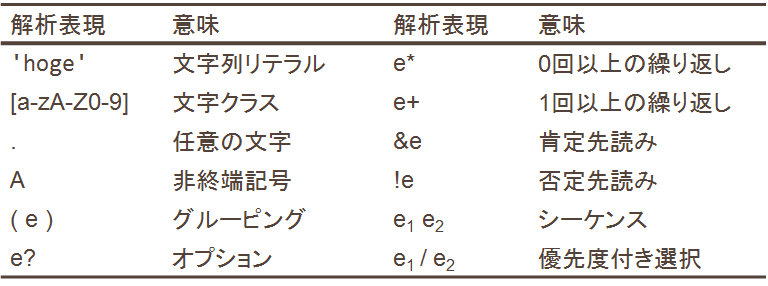
\includegraphics[width=70mm]{./fig/PEG}
 %      \caption{命令セット}
 %       \label{Ist_list}
    \end{center}
\end{figure}


\section{仮想マシン}

PEGはPackrat Parsing(PP論文)により線形時間に解析することができる。しかし、Packratは大きな入力に対して莫大なメモリ容量を使用するため、大きなデータの分析に向いていない。そこで、大きな入力を受理するため、MedeirosがPEGのためのVirtual Parsing Machineを提案した。
本研究で用いるバーチャルマシンはMedeirosが提案したバーチャルマシンをベースにする。

本研究で用いるVMは以下となる。

\begin{figure}[h]
    \begin{center}
        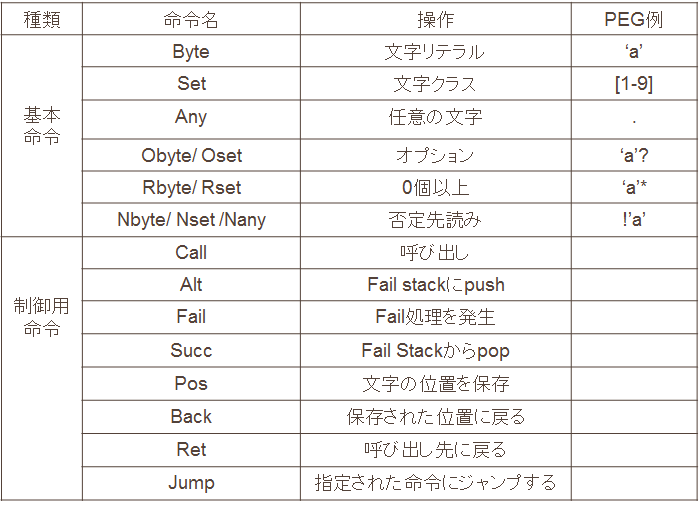
\includegraphics[width=70mm]{./fig/VM}
 %      \caption{命令セット}
 %       \label{Ist_list}
    \end{center}
\end{figure}

%Medeiosが提案したマシンは、次に実行する命令のアドレスを保存するプログラムカウンタ、文字列の現在位置を保存するレジスタ、そしてreturn addressとbacktrack entryを持っているスタックがある。Return addressはプリグラムカウンタのための値である一方、backtrack entryはアドレスと文字列のポジションの両方を持っている。

%基本的な命令は以下となる。\\
%Char x: 文字列の現在位置の文字と文字xをマッチさせ、成功すれば、文字列の位置を1つ増やす\\
%Any: 文字列の末端に到着しなければ、文字列の位置を一つ増やす。文字列の末端に到着すれば、失敗となる。\\
%Choice l : backtrack entryをスタックにプッシュする。lは別の選択肢との相対位置である。\\
%Jump l : 相対位置のlの命令にジャンプする\\
%Call l: 直後の命令アドレスをスタックにプッシュし、相対位置の命令にジャンプする\\
%Return : スタックから一つの命令アドレスをポップし、その命令にジャンプする\\
%Commit l : スタックから一つbacktrack entryを消し、そして相対位置のlの命令にジャンプする\\
%Fail:  スタックからbacktrack entryが出るまでポップし、そのbacktrack entryが新しい状態になる\\

%本研究で採用したバーチャルマシンは上記のバーチャルマシンを拡張したものである。
%扱いやすいために、ReturnスタックとFailスタックに分ける。Returnスタックは、Non-Terminalを呼び出すとき、プログラムレジスタPRの値を退避するためである。Failスタックはバックトラックの戻り値を保存するためである。\\

%MedeiosのVMに以下の命令を追加した。\\
%Set [x-y] : 文字列の現在位置の文字をASCIIの文字でのx以上y以下にマッチさせ、成功すれば、文字列の位置を一つ増やす。\\
 %OChar x, OSet[x-y] :文字リテラル、文字クラスのオプション(以下で述べる)\\ 
%Alt addr: 指定されたアドレスをFail stackにプッシュする\\
%RChar x, RSet[x-y] : 文字リテラル、文字クラスの0個以上\\
%First x addr: 最初の文字がxの場合、addrにジャンプする\\
%NChar x, NSet[x-y], NAny: 先読み\\
%Pos : 文字列の現在位置を専用レジスタに保存する\\
%Back: 保存された位置を文字列の現在位置にする\\

%\subsection{オプション}
%命令数を減らすために、以下の命令を定義する。\\
%OChar x: PEGの'x'?に対応する。文字列の現在位置の文字と文字xをマッチさせ、成功すれば、文字列の位置を1つ増やす。失敗した場合、次の命令に進む。\\
%OSet [x-y]: PEGの[x-y]?に対応する。Setと同様であるが、マッチが失敗した場合、次の命令に進む。\\

%本来であれば、例えば'PEGのx'?は以下の命令列が生成される。\\
%L1 Alt 3\\
%L2 Char x\\
%L3 Commit 1\\

%OChar x を使うことによって命令数を減らすことができた。

%\subsection{0個以上と先読み}
%同様に、以下の命令を定義する。\\
%RChar x : PEGの'x'* に対応する。文字列の現在位置の文字と文字xをマッチさせ、成功すれば、文字列の位置を1つ増やし、もう一回実行する。マッチされなくなれば、次の命令に進む。\\
%RSet [x-y] : PEGの[x-y]*に対応する。文字列の現在位置の文字をASCIIの文字でのx以上y以下にマッチさせ、成功すれば、文字列の位置を一つ増やし、もう一回実行する。マッチされなくなれば、次の命令に進む。\\
%NChar x: PEGの!'x'に対応する。Char xの逆であり、マッチされれば、失敗となる。マッチされなければ、成功となり、次の命令に進む。ただし、文字列の位置を変更しない。\\
%NSet [x-y] , NAny: それぞれPEGの![x-y]に対応する。NChar x と同様である。\\


\section{設計}

\subsection{全体図}

全体のシステムは図()となる。ホストとの通信はUbuntu OSとFPGAが可能にした、Xillybus社が提供しているXillybus IPコアを用いる。まずホストから命令列のバイトコードを受け取り、メモリに一時的に保存する。NezProcessorのメインメモリはFPGAに搭載しているブロックメモリで実装する。次に文字列をホストから受け取り、解析を行い、結果をホストを返す。

\begin{figure}[h]
    \begin{center}
        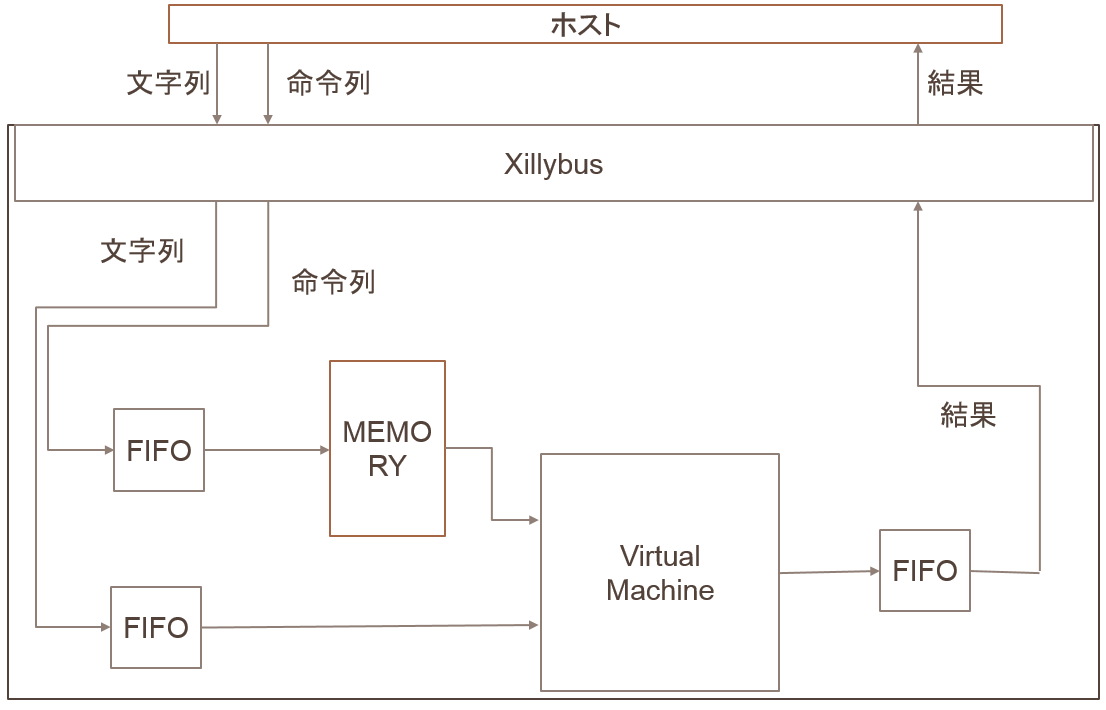
\includegraphics[width=70mm]{./fig/system}
      \caption{全体システム}
 %      \label{Ist_list}
    \end{center}
\end{figure}

Virtual Machineの全体図は図()となる。
まずは書き換え機能つきプログラムカウンタ(PC)がある。PCは次に実行すべき命令が格納されたメモリアドレスを指定する。プログムの実行に従って順次にインクリメントされ、ただし、分岐命令や割り込みが実行された場合は、分岐先のアドレスがPRに書き込まれる。\\
ReturnスタックとFailスタックがある。それぞれのスタックにスタックポインタがある。スタックポインタは、インクリメンタとディクリメンタを持っており、信号によってインクリメントやディクリメントが適時実行される。\\
命令を解読するデコーダやそれぞれの命令に特化した命令用回路がある。また、メモリから読み込んだ命令データ、FIFOから受け取った文字データはそれぞれ命令データレジスタ(IR)、文字データレジスタ(TR)に一時的に保存される。

\begin{figure}[h]
    \begin{center}
        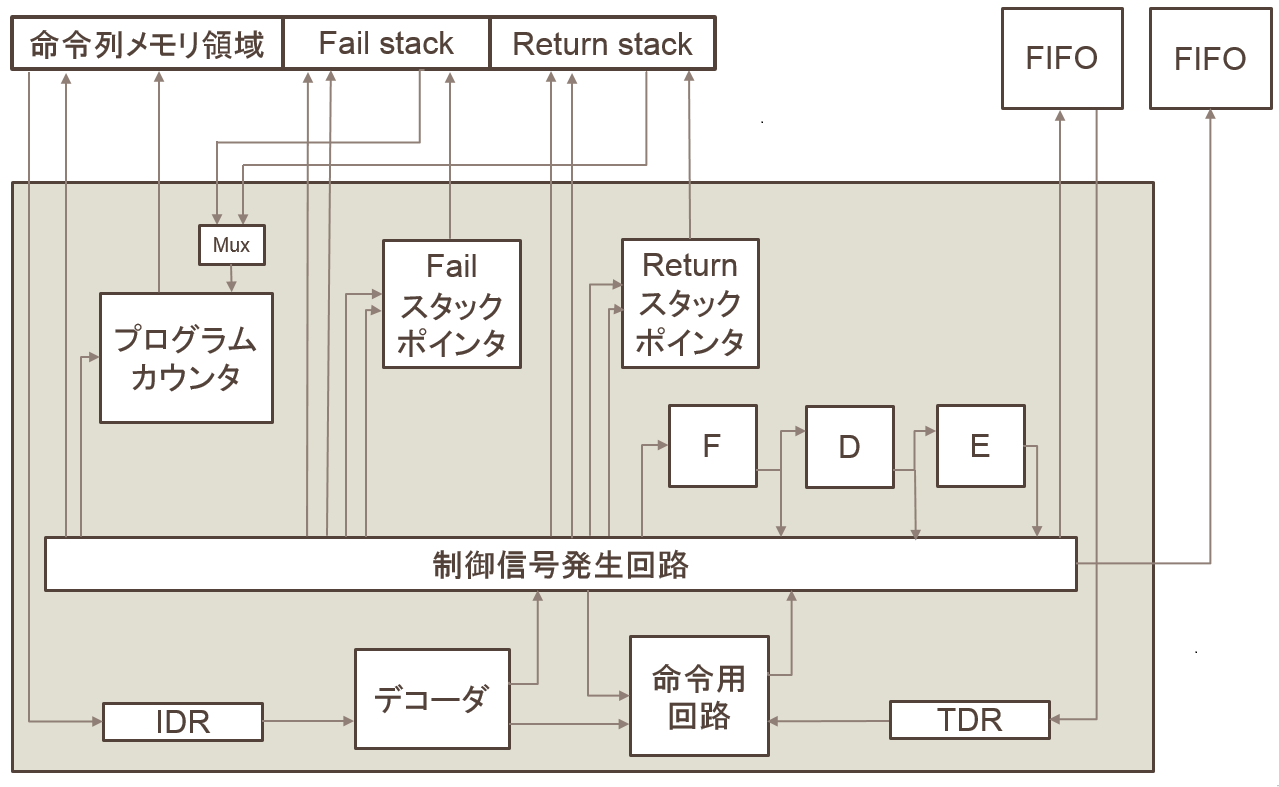
\includegraphics[width=70mm]{./fig/circuit}
       \caption{Virtual Machineの全体図 }
 %       \label{Ist_list}
    \end{center}
\end{figure}

NezProcessorの動作は、メモリからの命令の取り込み、解読、演算・データ転送といった一連の処理の繰り返しである。制御部の役割は、それを実現するための制御信号を適時生成して、演算回路やデータ転送回路に伝えることである。

NezProcessorでは、命令フェッチ、文字データ読み込み(F)、命令デコード(D)及び演算・データ転送を行う命令実行(E)という3つの状態がある。一般的に、命令フェッチは命令が格納されているメモリアドレスの設定、メモリデータレジスタへの読み込み、命令レジスタへの転送の3つの動作で構成される。しかし、本実装では、FPGAに搭載しているBlockRAMをメモリとして、使用するため、回路とメモリの距離が短く、命令フェッチは1クロックサイクルで実行できる。実際に、メモリアドレスは事前に設定しておき、読み出し信号がある場合、データをメモリデータレジスタを通さず、直接命令レジスタに転送される。D状態も1クロックサイクルで実行される。E状態は基本的に1クロックサイクルで実行されるが、Rbyte、Rsetや分岐命令の場合は命令用のフリップフロップがある。具体敵に()節に説明する。

どこ状態にあるかは制御信号生成回路によって制御される。状態F,D、Eに対して、3つのフリップフロップが直列に接続されている。プロセッサが起動するとき、Reset信号を一時的にハイレベルにする。スタート回路からハイレベルのフェッチ起動信号が出力される。Reset信号をローレベルに戻すと、次のクロックの立ち上がりで、状態Fに対するフリップフロップにフェッチ起動信号のハイレベル値が取り込まれる。同時にフェッチ起動信号はローレベルへ変換する。そのクロックの間、メモリへのread信号がハイレベルにする。

その次のクロックの立ち上がりで、状態Dに対するフリップフロップにハイレベルが取り込まれ、状態Fに対するフリップフロップの出力値はローレベルになる。そのクロックの間、IDRが持っている命令データがデコードされる。同様にして、その次のクロックサイクルでは、命令実行のための信号がハイレベルにして、命令を実行する。そして、次のクロックから新たな命令フェッチを実行する。


%\subsubsection{ハードウェア仕様}
%NezProcessorのワードは16ビットである。


%\subsubsection{命令の形式}
%第15ビットから第11ビットまではオペレーションフィールド(Opフィールド)であり、各命令に対応したコードが割り付けられる。第10ビットから第0ビットまでは命令の対象データとなる。命令によってこのデータの意味が異なる。
%Byte、Obyte、Rbyteの場合、文字である。
%Set、Oset、Rsetの場合、Setテーブルのインデックスとなる。Setテーブルは256行n列の行列であり、8ビットの文字を受け付けて、1ビットを出力する。
%Jump, Call, Alt の場合、命令アドレスを意味する。


%制御部はそのための制御信号生成回路と、命令を解読するためのデコーダから構成される。\\
%命令フェッチは命令が格納されているメモリアドレスの設定、メモリデータレジスタへの読み込み、命令レジスタへの転送の3つの動作で構成される。命令デコードでは、命令レジスタに取り込まれた命令のビットパターンから、どのような演算・データ転送を行うかを判断する。


%\subsubsection{命令フェッチ}
%NezProcessorでは、FPGAに搭載したBlockRAMをメインメモリとして、使う。FPGAでは、メモリを作るには、FFRAM、LUTRAM及びBlockRAMという3つの方法がある。大容量のメモリが必要な場合、BlockRAMはよく使われている。論理合成する際、メモリへの書き込み・書き出しが同期・非同期かによって、どのメモリを使うか、合成ツールが推論する。BlockRAMに推論されるために、書き込み・読み出しが同期でなければならない。
%前の命令でのEx状態で、次の命令アドレスの設定を行う。そして、F1状態でメモリにアクセスし、IRに転送する。Dec状態では、IRのデータをデコードする。この処理が繰り返される。
%\subsubsection{デコードと演算・データ転送}

%\subsubsection{制御信号生成回路の構成}
%NezProcessorの制御信号生成回路は、配線論理制御方式を採用している。配線論理制御方式は、目的の状態遷移をもつ順序回路によって制御を行う。図()に制御信号生成回路を示す。状態F1,Dec、Exに対して、3つのフリップフロップが直列に接続されている。

\subsection{各命令の実行}

\subsubsection{基本命令}

Byte命令実行のタイムチャートは図()に示す。F状態では、クロックの立ち上がりでread-ist信号がハイレベルになり、命令が格納されるメモリにアクセスし、データを命令レジスタ(IR)に転送される。アクセスアドレスはプログラムレジスタ(PR)から転送されたアドレスである。同時にread-text信号もハイレベルになり、FIFOから1文字を読み出し、文字レジスタ(TR)に転送される。

次のクロックの立ち上がりで、IRとCRのデータが確立され、このクロックサイクルでIRのデータがデコードされ、どの命令を実行するかが決まる。今回はByte命令用回路が実行されることになる。同クロックサイクルで、PRはインクリメントされ、メモリアクセス用のレジスタであるaddrにデータが転送される。

次のクロックサイクルの立ち上がりで、Byte命令用回路のトリガーであるByte-rがハイレベルになり、Byte命令用回路が実行される。IRが持っている文字データとCRの文字データが一致するならば、match信号がハイレベルになり、一致しなければ、fail信号がハイレベルになる。match信号及びfail信号は、制御信号生成回路の入力であり、match信号がハイレベルであれば、次のクロックから新たな命令フェッチを実行するように制御信号が生成される。一方、fail信号がハイレベルの場合、Fail処理を実行する制御信号が生成される。

\begin{figure}[h]
    %\begin{center}
    	\subfigure[Byte]{
        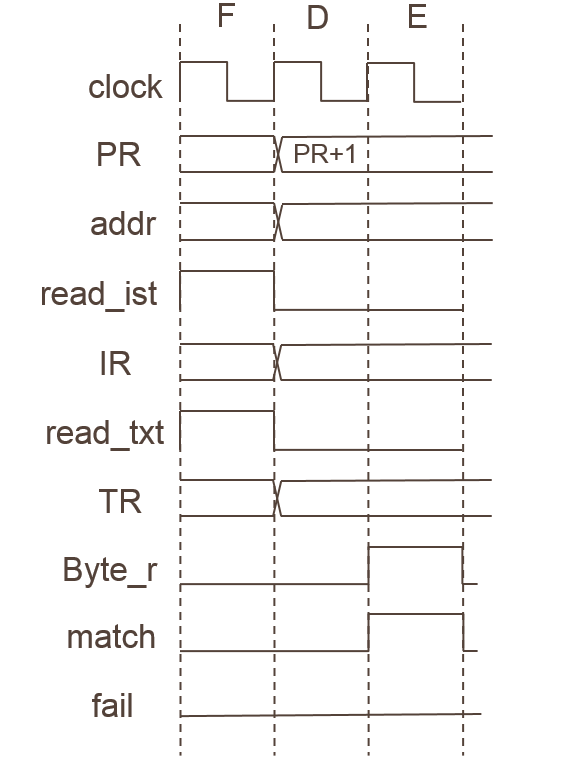
\includegraphics[width=30mm]{./fig/Byte}}
      \subfigure[Rbyte]{
        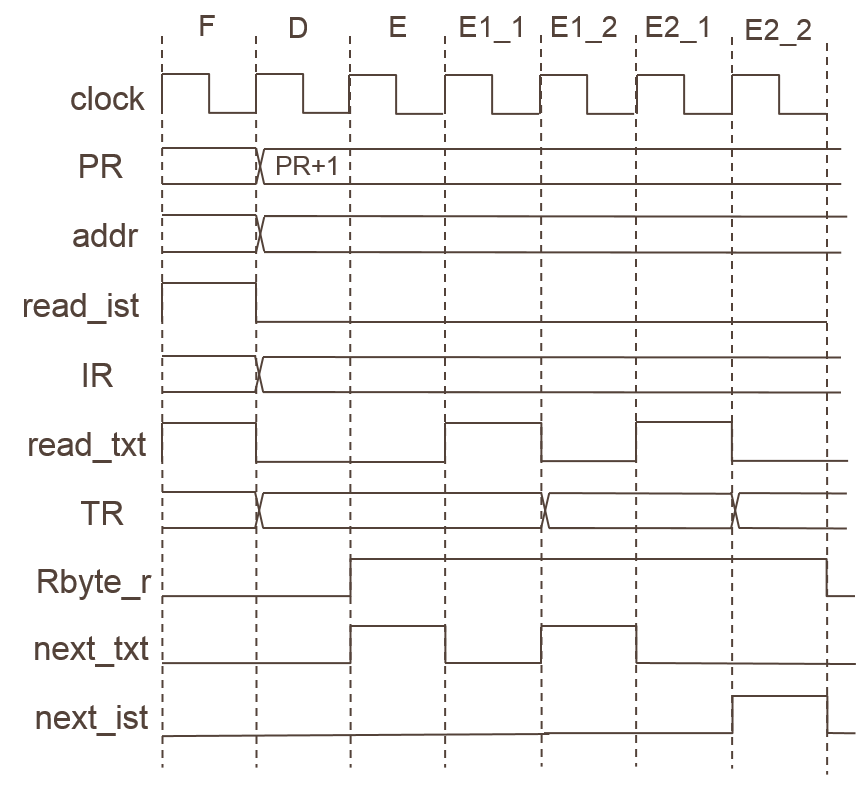
\includegraphics[width=45mm]{./fig/Rbyte}}
       \caption{基本命令実行のタイムチャート }
 %       \label{Ist_list}
    %\end{center}
\end{figure}

Rbyte命令実行では、F状態、D状態はByte命令と同様である。Ex状態では、IRが持っている文字データとTRの文字データが一致した場合、next-txt信号がハイレベルとなる。この場合、次のクロックサイクルの立ち上がりでread-txt信号がハイレベルとなり、FIFOから1文字を読み出す。次のクロックサイクルで、IRの持っている文字データと新たなTRの文字データを比較する。一致すれば、またFIFOから新たな文字を読み込まれる。IRの文字データとTRの文字データが一致しなくなるまで、この処理が繰り返される。この時、next-ist信号がハイレベルとなり、次のクロックから新たな命令フェッチを実行する。

Byte命令は、IRを持っている1文字のデータとTRの文字データを比較するのに対して、Set命令はTRの文字が複数の文字の中のどれかと一致するかを評価する命令である。Set命令を実行するために、Setテーブルを使う。Setテーブルは256ビットのデータの配列である。ASCII表のn番目の文字と一致したらマッチするという場合、nビット目を'1'にする。このようにして、与えられた文字をSetテーブルに照らし合わせて、そのビットの値は'1'であればマッチ成功、'0'であればマッチ失敗となる。\\

オプション命令(Obyte, Oset)も同様に実行されるが、文字消費信号を持っているところが違う。オプション命令はマッチ成功した場合、文字を消費し、マッチ失敗した場合、文字を消費しないが、Failにならず、次の命令に進む。先読み命令(NByte, NSet)の実行もByte,Set命令の実行と類似するが、文字を消費しない。\\

\subsubsection{分岐命令}
%分岐命令には、Jump命令がある。Jump命令の実行は、デコードを行うクロックサイクルDecと、次に実行すべき命令のアドレスをプログラムレジスタ(PR)に転送するクロックサイクルからなる。各クロックサイクルで生成された制御信号を以下に示す。

分岐命令には、Jump命令がある。Jump命令実行のタイムチャートは図()に示す。

E状態では、デコードの結果、Jump命令の実行のトリガーであるJump-rがハイレベルになり、プログラムレジスタのトリガーであるPR-lat信号もハイレベルになる。この場合、インクリメントのトリガーであるPR-incはローレベルであるため、ジャンプ先のアドレスを持っているPC-data-inの値はPRに置き換える。次のクロックサイクルでPRの値が少し遅れてメモリアドレスレジスタaddrに転送される。また、次のクロックサイクルの立ち上がりで新たな命令フェッチが始まる。


\begin{figure}[h]
    \begin{center}
        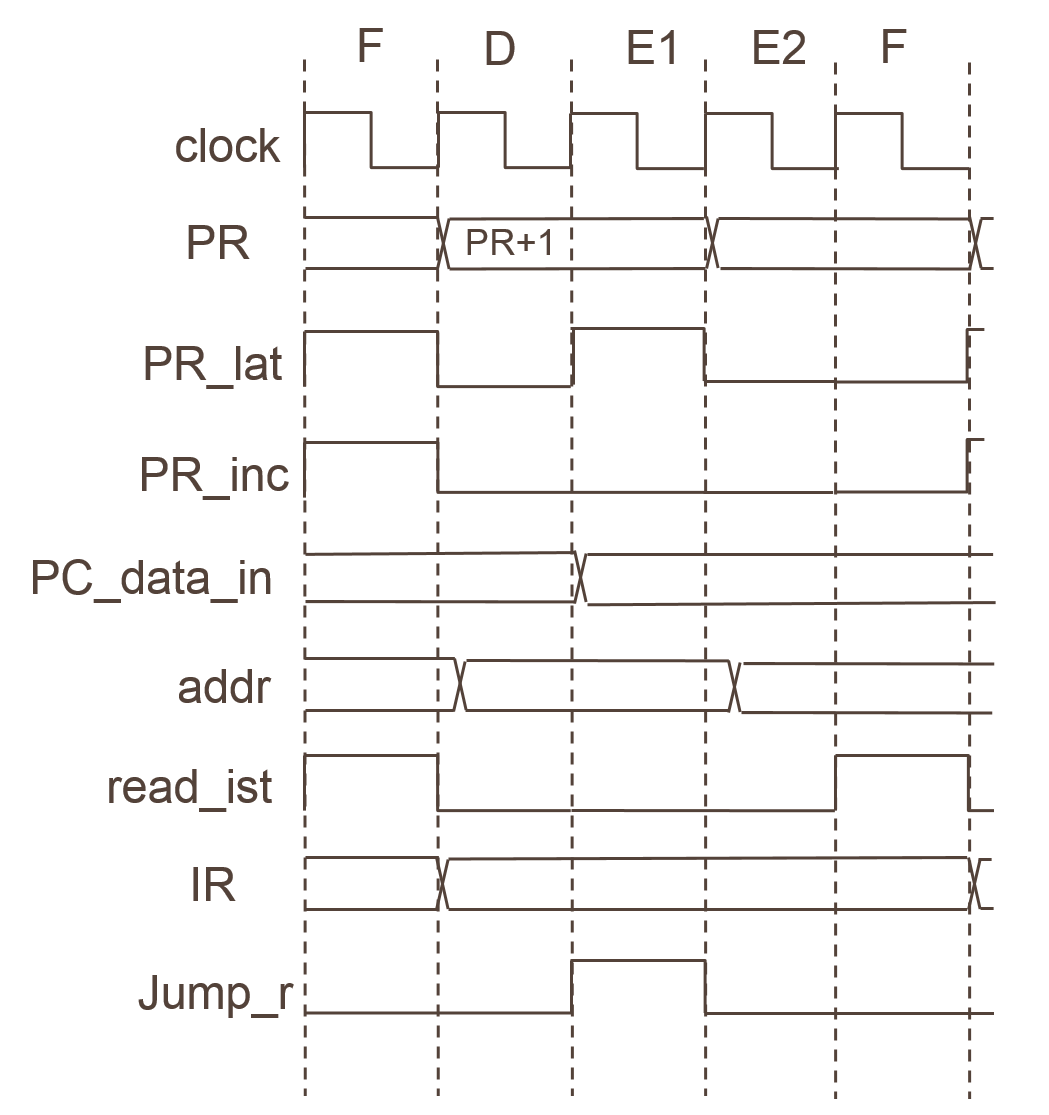
\includegraphics[width=50mm]{./fig/Jump}
       \caption{Jump命令実行のタイムチャート}
 %       \label{Ist_list}
    \end{center}
\end{figure}

\subsubsection{スタック操作命令}
スタック操作命令には、Call、Alt、Return、Succがある。

Non-Terminalを呼び出す命令がCall命令であり、それを呼び出したプログラムへ実行制御を返すのがReturn命令である。Call命令は、プログラムレジスタPRの値をReturnスタックにプッシュダウンして退避させ、Non-Terminalの先頭番地であるアドレスをPRに転送する。Call命令の実行はJump命令と類似しており、ただ新たなアドレスをPRに転送している同時に、Returnスタックにプッシュダウンを行う。
Return命令は、Call命令によってスタックに退避したNon-Terminalからの戻り番地をポップアップしてPRへ転送する。これによって、Non-Terminalを呼び出したプログラムへ実行制御が返される。
Return命令実行のタイムチャートは図()に示す。

\begin{figure}[h]
    \begin{center}
        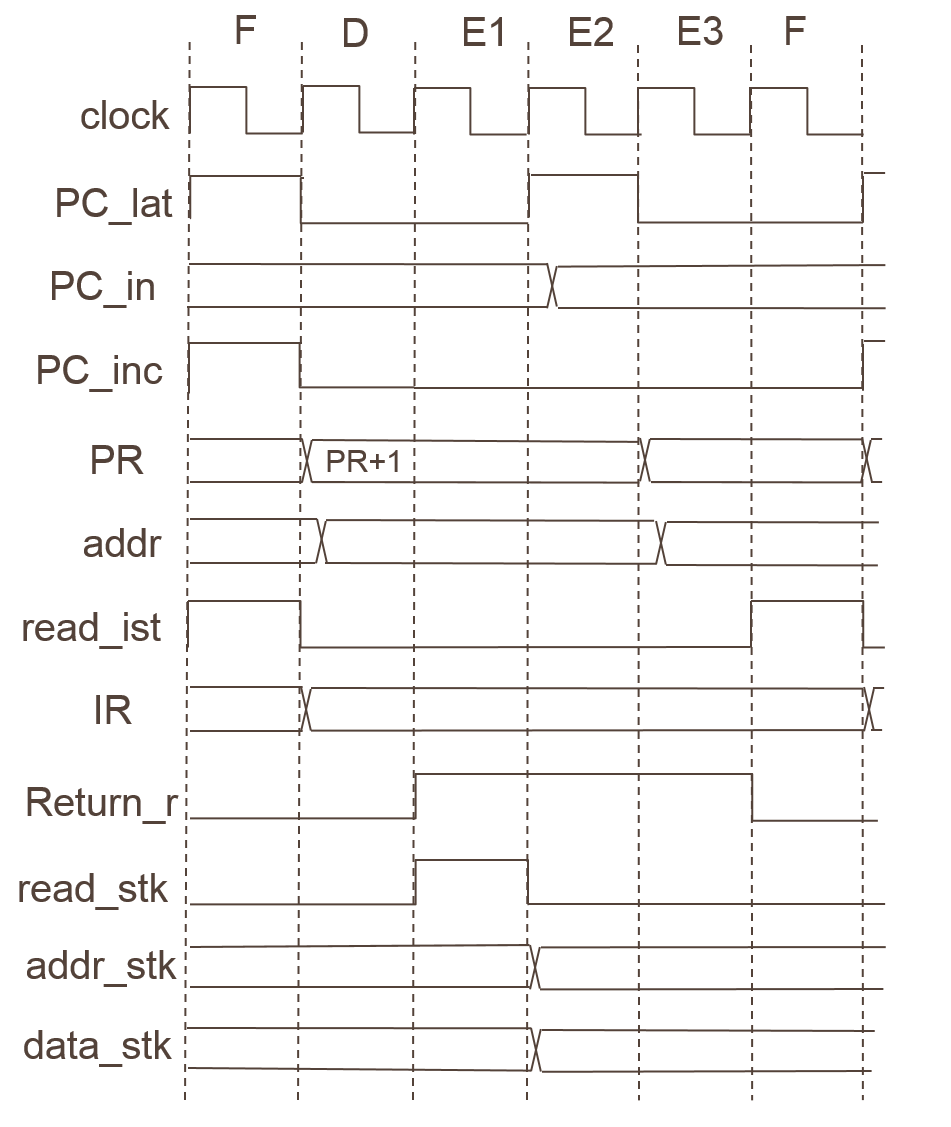
\includegraphics[width=50mm]{./fig/Return}
       \caption{Return命令実行のタイムチャート}
 %       \label{Ist_list}
    \end{center}
\end{figure}

E1状態のクロックサイクルの立ち上がりで、Return命令実行のトリガーであるReturn-r信号がハイレベルになる。同クロックサイクルでReturnスタックの読み出し信号であるread-stkがハイレベルになり、データをdata-stkに転送される。次のクロックサイクルでPRの書き換えデータPC-data-inに少し遅れて転送される。次のクロックサイクルの立ち上がりでPRの新たなアドレスが確立し、少し遅れて命令のアドレスであるaddrに転送される。次に新たな命令フェッチが始まる。



%その実行ステップはデコードを行うクロックサイクルDecと、メモリスタックにデータをプッシュダウンするクロックサイクルEx、及びPRにポップアップされた命令アドレスへの転送を行うクロックサイクルからなる。同様に、スタックポインタのインクリメント及びスタックメモリアドレスの設定は既に実行済みである。各クロックサイクルで生成される制御信号は以下に示す(図)。

%Return命令はSucc命令と類似しているが、両者の違いは、Succ命令はFailスタックからポップアップした値を捨てるのに対して、Return命令はポップアップした値をPRへ転送する点である。

%Alt命令の実行ステップは、デコードを行うクロックサイクルDecと、メモリスタックにデータをプッシュダウンするクロックサイクルExからなる。スタックポインタのインクリメント及びスタックメモリアドレスの設定は、前回のスタックプッシュが終わり次第、すでに実行された。このため、Call命令は3つのクロックサイクルで実行が可能になる。クロックサイクルExが終ったら、新たな命令フェッチが実行される同時に、スタックポインタのインクリメントとスタックメモリアドレスの設定も実行される。各クロックサイクルで生成された制御信号を以下に示す。
%Succ命令も同様である。



%\subsubsection{割り込み}
PEGでは、バックトラックがある。バックトラックは、Choiceがある場合、ある選択肢でマッチが失敗した場合、前の状態に戻り、別の選択肢を評価する仕組みである。Choiceがある場合、選択肢を評価する前に、バクトラックが起こるときの戻り先をFailスタックにプッシュダウンされる。どこかでマッチが失敗したら、バックトラック処理が実行される。

Failスタックを操作する命令はAlt命令とSucc命令がある。Alt命令はFailスタックにデータをプッシュダウンし、Succ命令はFailスタックからデータをポップアップする。ALt命令とSucc命令の動作はCall命令、Return命令と類似しているが、両者の違いはALt命令とSucc命令がスタックを操作するだけで、PRにデータを転送しない点である。

一方、どこかでマッチが失敗した場合、バックトラック処理が実行される。バックスタック処理はReturn命令の実行と類似している。

%バックトラック処理では、Failスタックからポップアップするクロックサイクル、ポップアップされた値をPRへ転送するクロックサイクルからなる。バックトラック処理で生成される制御信号は以下に示す(図)。

\section{性能評価}

%実装環境\\

%C言語版との性能比較


\section{まとめ}

\ack %% 謝辞
%本論文は私が横浜国立大学理工学部数物電子情報系学科電子情報システムEPに在籍中の研究成果をまとめたものである。
%本論文を執筆するにあたり、横浜国立大学工学部電子情報工学科准教授である倉光君郎先生
%には、指導教官として研究の方針をご指導頂きました。また、FPGAについて様々なアドバイスをしていただいた株式会社イーツリーズ・ジャパンの三好健文様、資料作成に付き合っていただいた関口渚、森谷鴻平、山口真弥、本多峻、田村健介、須藤建、千田忠賢先輩及びB4のみなさんに深く感謝の意を表します。\\
%\\
%加えて、私の学生生活を長きにわたって見守って下さった私の家族に深く感謝致します。

%\bibliographystyle{sieicej}
%\bibliography{myrefs}
\begin{thebibliography}{99}% 文献数が10未満の時 {9}
\bibitem{}
\end{thebibliography}

\appendix
\section{}

\begin{biography}
\profile{}{}{}
%\profile{会員種別}{名前}{紹介文}% 顔写真あり
%\profile*{会員種別}{名前}{紹介文}% 顔写真なし
\end{biography}

\end{document}








